\section{动态不均衡特征分析}
\label{section:background}

\begin{figure}[t]
    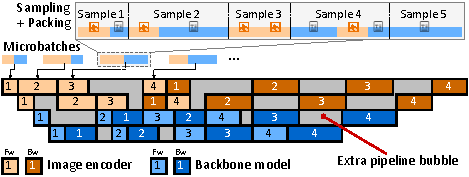
\includegraphics[width=1\columnwidth]{figures/svg/imbalanced_pipeline.pdf}
    \caption{
        动态不均衡影响示意图。
    }
    \label{figure:imbalanced-pipeline}
\end{figure}

\begin{figure*}[!t]
    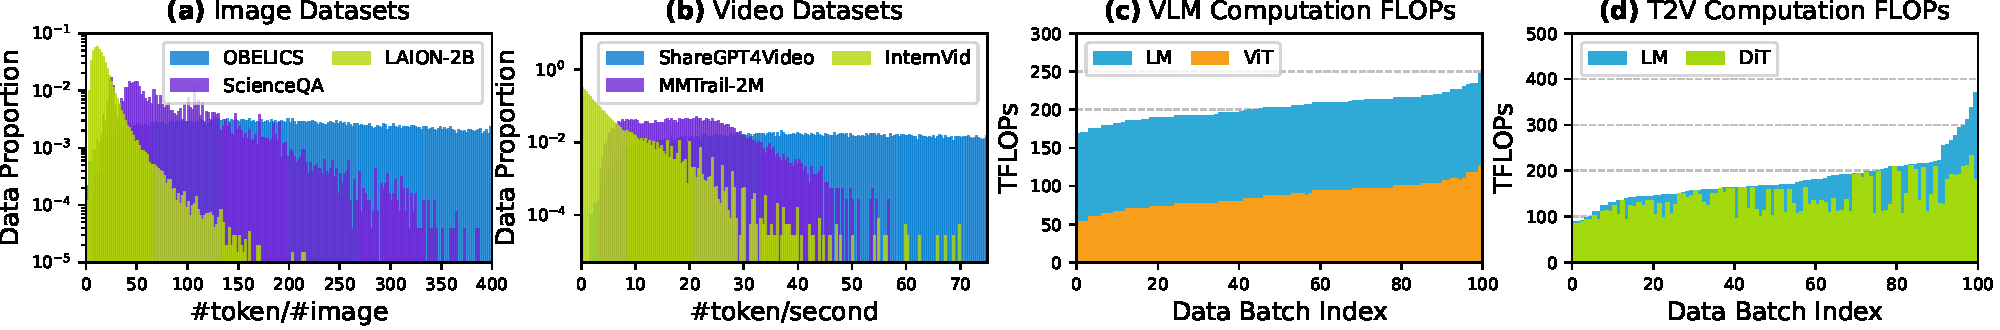
\includegraphics[width=1\textwidth]{figures/data_distribution.pdf}
    \caption{
        \textbf{(a--b)} OBELICS~\cite{obelics-arxiv23}、LAION-2B~\cite{laion5b-nips22} 和 ScienceQA~\cite{scienceqa-nips22} 数据集中每幅图像对应的 token 分布，以及 ShareGPT4Video~\cite{share-gpt4-video-arxiv24}、InternVid~\cite{internvid-arxiv23} 和 MMTrail-2M~\cite{mmtrail-arxiv24} 视频数据集中每秒视频对应的 token 分布。Y 轴表示归一化数据比例。\linebreak
        \textbf{(c--d)} VLM 12B（表~\ref{table:model-setup} 中的 VLM-S）和 T2V 13B（表~\ref{table:model-setup} 中的 T2V-S）模型在 100 个已打包数据批次上的计算需求。批次（X 轴）按计算成本升序排列，浮点运算量（Y 轴）以 teraFLOPs（TFLOPs）计量。
    }
    \label{figure:data-distribution}
\end{figure*}

\subsection{大多模态模型}

多模态模型长期以来一直试图通过学习统一的语义表示来连接异构模态~\cite{modality-bridge-arxiv23}。
早期基于 CLIP 的多模态模型~\cite{clip-arxiv21} 开创了双编码器架构（例如图像使用 ViT、文本使用 BERT），并利用对比损失~\cite{simclr-icml20} 在共享语义空间中对齐跨模态嵌入。

大多模态模型（LMM）的出现标志着一次范式转变：其目标从表示对齐扩展到多模态生成能力。这一演进由大规模、基于 Transformer 的架构整合所推动，包括大语言模型（LLM）、视觉 Transformer（ViT）和扩散 Transformer（DiT）。
如\figref{figure:mm-vs-lmm}所示，LMM 使用模态适配器将编码器与骨干模型集成。随后，骨干模型通过自回归过程或扩散机制生成输出表示，再由专用模态解码器将这些表示转换为文本、音频和图像等人类可感知的形式。
与基于 CLIP 的模型相比，LMM 的可扩展生成式架构显著拓宽了所支持任务的范围。
例如，在一个 LMM 中（\figref{figure:mllm-demo}），用户可在同一查询中交错使用文本、图像和视频，并通过追加后续问题反复细化查询，形成多轮对话~\cite{gpt4o-image-generation,gemini-3-2025,dialog-gen-arxiv24}。
LMM 可以文本或语音形式响应~\cite{step-audio-arxiv25}，还可使用扩散模块生成图像~\cite{moviegen-arxiv24,step-t2v-arxiv25,hunyuan-dit-arxiv24}。

\heading{LMM 训练}
大型 Transformer 模型通常采用数据并行（DP）、流水线并行（PP）和张量并行（TP）等三维分布式方案进行训练~\cite{megatron-lm-arxiv20}。
流水线并行将模型层划分为多个\emph{模型块}，并放置在不同机器（即流水线秩）上。
每个模型块都可以执行前向和反向阶段计算。
数据批次被拆分为更小的微批次，并通过点到点（P2P）通信在流水线阶段之间传递。
